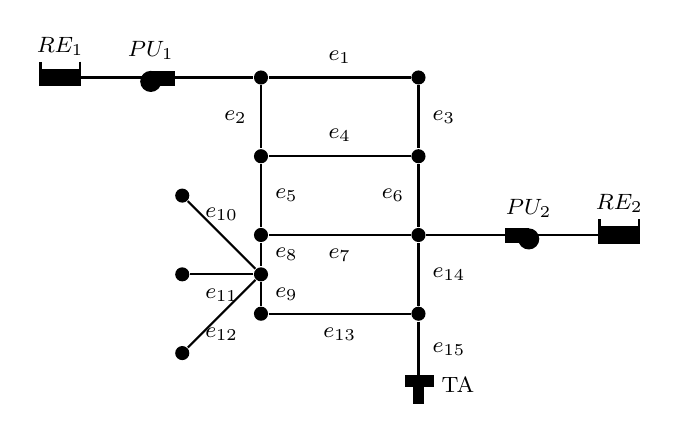
\begin{tikzpicture}[semithick,state/.style ={ draw,shape=circle,scale=0.95}]

\node[circle,fill,inner sep=1.8pt,label=above : \footnotesize$$] (A) at (0,0) {};
\node[circle,fill,inner sep=1.8pt,label=above : \footnotesize$$] (B) at (2,0) {};
\node[circle,fill,inner sep=1.8pt,label= left: \footnotesize$$] (C) at (0,-1) {};
\node[circle,fill,inner sep=1.8pt,label= right: \footnotesize$$] (D) at (2,-1) {};
\node[circle,fill,inner sep=1.8pt,label= above right: \footnotesize $$] (E) at (2,-2) {};
\node[circle,fill,inner sep=1.8pt,label= above left: \footnotesize$$] (F) at (0,-2) {};
\node[circle,fill,inner sep=1.8pt,label= below : \footnotesize$$] (G) at (0,-3) {};
\node[circle,fill,inner sep=1.8pt,label=  right: \footnotesize$$] (H) at (0,-2.5) {};
\node[circle,fill,inner sep=1.8pt,label=  right: \footnotesize$$] (I) at (2,-3) {};
\node[circle,fill,inner sep=1.8pt,label=  above: \footnotesize$$] (J) at (-1,-1.5) {};
\node[circle,fill,inner sep=1.8pt,label=  above: \footnotesize $$] (M) at (-1,-2.5) {};
\node[circle,fill,inner sep=1.8pt,label=  above: \footnotesize $$] (L) at (-1,-3.5) {};



\draw [thick] (A) -- node[above  =0.05 cm] {\footnotesize$e_1$}  (B);
\path (A) edge [thick]  node[left  =0.05 cm] {\footnotesize$e_2$} (C);
\path (B) edge [thick] node[right  =0.05 cm] {\footnotesize$e_3$} (D);
\path (C) edge [thick] node[above  =0.05 cm] {\footnotesize$e_4$} (D);
\path (C) edge [thick] node[right  =0.05 cm] {\footnotesize$e_5$} (F);
\path (D) edge [thick] node[left  =0.05 cm] {\footnotesize$e_6$} (E);
\path (E) edge [thick] node[below  =0.05 cm] {\footnotesize$e_7$} (F);
\path (F) edge [thick] node[right  =0.05 cm] {\footnotesize$e_8$} (H);
\path (H) edge [thick] node[right  =0.05 cm] {\footnotesize$e_9$} (G);
\path (H) edge [thick] node[above  =0.05 cm] {\footnotesize$e_{10}$} (J);
\path (H) edge [thick] node[below  =0.05 cm] {\footnotesize$e_{11}$} (M);
\path (H) edge [thick] node[below  =0.05 cm] {\footnotesize$e_{12}$} (L);
\path (G) edge [thick] node[below  =0.05 cm] {\footnotesize$e_{13}$} (I);
\path (E) edge [thick] node[right  =0.05 cm] {\footnotesize$e_{14}$} (I);

%PU2
\node[circle,fill,inner sep=2.7pt,label= above : \footnotesize $ PU_2$] (I) at (3.4,-2.05) {};
\draw [thin,fill] (3.1,-1.92) rectangle (3.4,-2.1);


\begin{scope}[xscale=-1,yscale=1]
%PU1
\node[circle,fill,inner sep=2.7pt,label= above : \footnotesize $ PU_1$] (I) at (3.4-2,-2.05+2) {};
\draw [thin,fill] (3.1-2,-1.92+2) rectangle (3.4-2,-2.1+2);

\end{scope}

\draw [thick](2.1,-2) -- (3.1,-2);
\draw [thick, fill] (1.84,-3.79) rectangle (2.18,-3.92);
\draw [thick,fill] (1.95,-3.92) rectangle (2.06,-4.13);
\draw [thick](2,-3.1) -- node[right  =0.05 cm] {\footnotesize$e_{15}$}(2,-3.8);
\node at (2.5,-3.9) {\footnotesize TA};


\draw [thick](-0.1,0) -- (-1.1,0);


\draw [thick](3.5,-2) -- (4.3,-2);
\draw [thick](-1.5,0) -- (-2.3,0);
\draw [thick](-2.3,0.2) -- (-2.3,-0.1) -- (-2.8,-0.1) -- (-2.8,0.2);
\draw [thick,fill] (-2.8,0.1) rectangle (-2.3,-0.1);
\draw [thick](4.3,-1.8) -- (4.3,-2.1) -- (4.8,-2.1) -- (4.8,-1.8);
\draw [thick,fill] (4.3,-1.9) rectangle (4.8,-2.1);
\node at (-2.55,0.4) {\footnotesize $RE_1$};
\node at (4.55,-1.6) {\footnotesize $RE_2$};
\end{tikzpicture}